% Add "answers" option to print the answers
\documentclass[addpoints]{exam}

\usepackage[utf8]{inputenc}
\usepackage{calc}
\usepackage{listings}
\usepackage{xcolor}
\usepackage{xspace}

\definecolor{codegreen}{rgb}{0,0.6,0}
\definecolor{codegray}{rgb}{0.5,0.5,0.5}
\definecolor{codepurple}{rgb}{0.58,0,0.82}

\lstdefinestyle{Cstyle}{
    commentstyle=\color{codegreen},
    keywordstyle=\color{magenta},
    numberstyle=\tiny\color{codegray},
    stringstyle=\color{codepurple},
    basicstyle=\ttfamily\small,
    breakatwhitespace=true,
    breaklines=true,
    captionpos=b,
    keepspaces=true,
    numbers=left,
    numbersep=5pt,
    showspaces=false,
    showstringspaces=false,
    showtabs=false,
    tabsize=4
}

\lstset{style=Cstyle}

% \makebox[\textwidth]{Name:\enspace\hrulefill}
%
% \vspace{5mm}
%\makebox[\textwidth]{Instructor’s name:\enspace\hrulefill}

\newcommand{\truefalse}
{		\begin{checkboxes}
			 \choice True
			 \choice False. Explanation:
		\end{checkboxes}
		\vspace{10pt}
}

\newcommand{\answerspace}[1]
{
	\ifprintanswers
	\else
		\setlength{\mylength}{10pt}%
		%\noindent\rule{\mylength}{20pt}
		%\vspace{\fpeval{1.2*(#1)}}
		\vspace{#1\mylength}
	\fi
}
\newlength{\mylength}

\newcommand\pf[1]{\textcolor{red}{PF: #1}}
\newcommand\am[1]{\textcolor{blue}{AM: #1}}

\newcommand{\answer}[1]{\begin{solution}{#1}\end{solution}}
\newcommand{\ra}{$\rightarrow$\xspace}


\usepackage{color}
\usepackage{lastpage}
\usepackage{verbatim}
\usepackage{fancyvrb}
\usepackage{graphicx}
\usepackage{float}
\usepackage{minted}
\usepackage{multicol}
\usepackage{amsmath}

\usepackage[svgnames]{xcolor}
\usepackage[colorlinks=true, allcolors=MidnightBlue]{hyperref}

% For those sweet, sweet acmart fonts.
\usepackage[T1]{fontenc}
\usepackage[tt=false, type1=true]{libertine}
\usepackage[varqu]{zi4}                  % Inconsolata for \ttfamily

% Eliminate extraneous spacing on itemize, description, etc.
\usepackage{enumitem}
\setlist{nosep}

\newcommand{\Code}[1]{\mintinline{python}{#1}}
\newcommand{\nonAnswerNewPage}{\ifprintanswers \vfill \else \newpage \fi}

% Macros for the symbolic and concolic execution questions
\newcommand{\StateQ}[5]{[\Code{x}$\mapsto$\Code{#1},
  \Code{y}$\mapsto$\Code{#2}, \Code{a}$\mapsto$\Code{#3},
  \Code{b}$\mapsto$\Code{#4}, \Code{result}$\mapsto$\Code{#5}]}
\newcommand{\StateS}[5]{[\Code{x}$\mapsto #1$, \Code{y}$\mapsto #2$,
  \Code{a}$\mapsto #3$, \Code{b}$\mapsto #4$,
  \Code{result}$\mapsto #5$]}

\renewcommand{\solutiontitle}{\noindent\textbf{Solution sketch: }}
\definecolor{SolutionColor}{rgb}{0.8,0.9,1}

\cfoot{Page \thepage\ of \pageref{LastPage}}
\rhead{Initials: \rule{20mm}{0.4pt}}

%%%%%%%%%%%%%%%%%%%%%%%%%%%%%%%%%%%%%%%%
\begin{document}
\fvset{numbers=left,numbersep=3pt}
\thispagestyle{empty}

\begin{center}
  {\LARGE{\textbf{CS 408: Homework 5}}}\\
  \vspace*{5pt}
  {\Large Deadline: Friday, November 6 \textbf{at 6PM}}\\
  \vspace*{10pt}

  \fbox{
    \fbox{\parbox{6in}{\centering
        \begin{itemize}
        \item The homework is open notes, open book.
        \item Please upload an annotated version of this pdf, ensuring
          that each answer fits in the box following each question.
        \item All solutions must be \textbf{handwritten}; typed work
          will not receive any credit. You may annotate the pdf
          directly, no need to print out and rescan.
        \item No AI tools allowed.
        \item If a question asks for code, you do not need to
          reproduce Hypothesis's syntax exactly, but make sure that we
          can clearly identify what each strategy produces and what
          each property is testing.
        \item No collaboration with your peers of any kind allowed on
          this homework.
        \item Homeworks are due at \textbf{6PM}. Anything submitted
          after \textbf{6PM} will not be accepted.
        \item Provide complete and clear but concise answers. Clearly
          explain your answers where required.
	\end{itemize}
      }}}
\end{center}

\begin{center}
	\makebox[0.6\textwidth]{
		\combinedgradetable[h][questions]
	}
\end{center}
%\begin{center}\combinedgradetable[h][questions]\end{center}

\vspace{5mm}
\begin{center}
\makebox[\textwidth]{\textbf{Name (please print)}: \rule{100mm}{0.8pt} }
\end{center}

\begin{questions}

%% =====================================================================
%% Q1+2 -- Delta Debugging
%% =====================================================================

\question Suppose that we have the test input ``Hello World!'',
  and a test that fails on any string that contains at least one 'o'
  and at least one 'd'.

  \begin{parts}
    \part[10]
      Show the \textbf{first 10} test inputs produced by the delta
      debugging algorithm (\Code{ddmin}) discussed in class, omitting
      any repeated inputs and noting whether each of those test inputs
      triggered a failure or not. %
      \begin{solutionorbox}[3.5in]
        \begin{enumerate}
        \item ``Hello '' (no failure)
        \item ``World!'' (failure)
        \item ``Wor'' (no failure)
        \item ``ld!'' (no failure)
        \item ``Wo'' (no failure)
        \item ``rl'' (no failure)
        \item ``d'' (no failure)
        \item ``!'' (no failure)
        \item ``rld!'' (no failure)
        \item ``Wod!'' (failure)
        \end{enumerate}
      \end{solutionorbox}

    \part[2] Give the \textbf{final input} returned by the
      \Code{ddmin} algorithm on this input, again noting whether or
      not it failed.
  \begin{solutionorbox}[.75in]
    Final result: ``od'' (failure)
  \end{solutionorbox}
\end{parts}

\nonAnswerNewPage
\question All of the test case minimization algorithms we have seen in
  class assume access to a deterministic test oracle, i.e., one
  that either \emph{always} fails or \emph{always} succeeds on the
  same test input.
  \begin{parts}
  \part[2] What is an example of a testing scenario where this
    assumption does not hold, i.e., the test oracle is \emph{flaky},
    and the same input sometimes passes and sometimes fails? %
    \begin{solutionorbox}[2in]
      Consider a program under test that spawns several concurrent
      processes which update a shared variable \Code{x} and which do
      not use an appropriate locking discipline. In this scenario,
      there is a data race on \Code{x}, and the test oracle's answer
      may depend on both the test input and the scheduler, e.g., if
      the failure is only triggered by a specific final value of
      \Code{x}.
      \end{solutionorbox}

    \part[4] Would the outputs of any of the minimization algorithms
      we've seen be affected in a meaningful way if they use a flaky
      test oracle? Which ones, and how? %
    \begin{solutionorbox}[2.5in]
      Indeed! \textbf{All} of the algorithms we've seen before make
      decisions based on whether a candidate input triggers a failure:
      the straightforward algorithm from the project only deletes a
      byte from a test input if the SUT still fails after doing so,
      while \Code{ddmin} only recurses on a modified input when it
      fails. For all of these algorithms, a flaky test oracle can
      cause the algorithm to produce a non-minimal failing input.  In
      the worst case scenario, a flaky test oracle could cause the
      minimizer to return the original input unchanged, even though a
      simpler version of the failing input exists.
    \end{solutionorbox}

  \part[2] Propose one concrete strategy for dealing with flaky tests
    when using one of the algorithms from your previous answer, and
    briefly explain how this strategy would improve the reliability
    of the algorithm. %
    \begin{solutionorbox}[2in]
      One simple solution is to run each test multiple times and
      recursively minimize that input if \textit{any} of those tests
      fail.
    \end{solutionorbox}

  \end{parts}

  \nonAnswerNewPage
%% =====================================================================
%% Q2 -- Symbolic Execution
%% =====================================================================

\question Consider the following program:

  \begin{minted}{python}
def fun(a: int, b: int, c: int) -> None:
    x = 100
    if a >= 0:
        x = 50
    if b + c > 0:
        x += c
        if x < 70:
            x += a
    return
\end{minted}

\begin{parts}
\part[10] Provide the \textit{execution tree} produced by symbolic
  execution for this program. The nodes of this tree should be
  labelled with the corresponding control flow point and the symbolic
  state\footnote{On all of your answers for this question, please name
    symbolic variables using the convention $s_0, s_1, s_2, ...$.}
  before that basic block or condition is executed: using the format
  L2: $[x\mapsto s_1; z \mapsto s_4; \ldots]$. The root of the tree
  should appear at the top of the diagram. The outgoing edges of
  decision nodes should be labelled with the corresponding path
  conditions, and the labels on its left and right subtrees should
  correspond to the true and false branches of the original
  \texttt{if} statement, respectively. Please make sure the image is
  legible: we will deduct points if we can't decipher your
  handwriting.

  %
  \begin{solutionorbox}[5in] %
    \begin{center}
      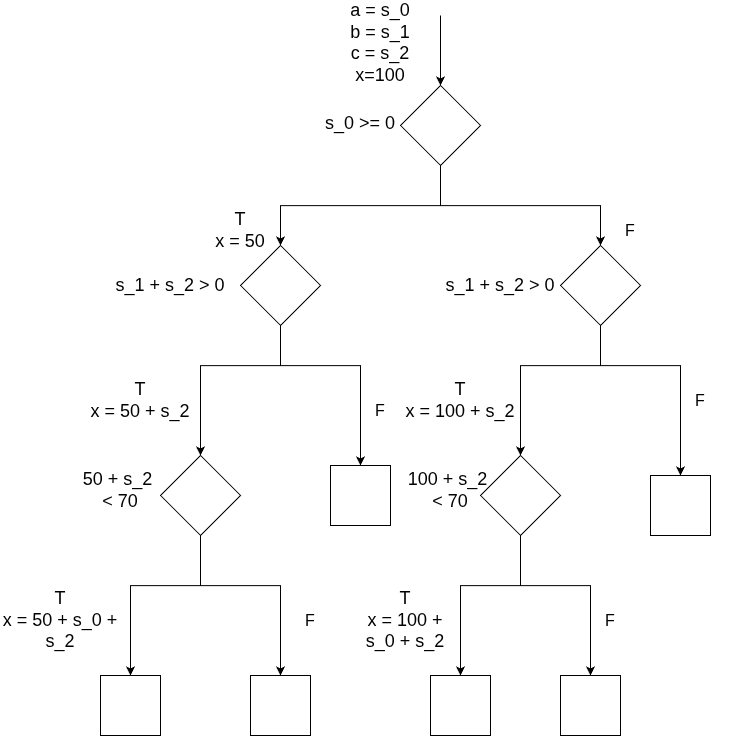
\includegraphics[scale=0.40]{q1_graph_answer.png}
    \end{center}
  \end{solutionorbox}

  \nonAnswerNewPage

\part[2] Please list the path condition corresponding to an execution
  in which the conditions of all three \texttt{if} statements are
  \textbf{true}: (\textbf{true}, \textbf{true}, \textbf{true})
  % \pf{Apply the changes I made here to the other relevant subquestions.}
  % \am{Applied the changes.}
  %
  \begin{solutionorbox}[1in]
    ($s_0 \geq 0) \wedge (s_1 + s_2 > 0) \wedge (50 + s_2 < 70)$
  \end{solutionorbox}

\part[2] Please list the path condition corresponding to an execution
  in which the conditions of the first two \texttt{if} statements are
  \textbf{true}, and the last one is \textbf{false}: (\textbf{true},
  \textbf{true}, \textbf{false})
  %
  \begin{solutionorbox}[1in]
    $(s_0 \geq 0) \wedge (s_1 + s_2 > 0) \wedge \neg (50 + s_2 < 70)$
    \textbf{OR}
    $(s_0 \geq 0) \wedge (s_1 + s_2 > 0) \wedge (50 + s_2 \geq 70)$
    \end{solutionorbox}

\part[2] Please list the path condition corresponding to an execution
  in which the condition of the first \texttt{if} statement is
  \textbf{true}, and the second is \textbf{false}: (\textbf{true},
  \textbf{false})
  %
  \begin{solutionorbox}[1in]
    ($s_0 \geq 0) \wedge \neg (s_1 + s_2 > 0)$
    \textbf{OR}
    ($s_0 \geq 0) \wedge (s_1 + s_2 \leq 0)$
\end{solutionorbox}

\part[2] Please list the path condition corresponding to an execution
  in which the condition of the first \texttt{if} statement is
  \textbf{false}, and those for the other two are \textbf{true}:
  (\textbf{false}, \textbf{true}, \textbf{true})
  %
  \begin{solutionorbox}[1.5in]
    $\neg (s_0 \geq 0) \wedge (s_1 + s_2 > 0) \wedge (100 + s_2 < 70)$
    \textbf{OR}
    $(s_0 < 0) \wedge (s_1 + s_2 > 0) \wedge (100 + s_2 < 70)$
\end{solutionorbox}

\part[2] Please list the path condition corresponding to an execution
  in which the condition of the first \texttt{if} statement is
  \textbf{false}, the second is \textbf{true}, and the third is
  \textbf{false}: (\textbf{false}, \textbf{true}, \textbf{false})

  %
  \begin{solutionorbox}[1.5in]
    $\neg (s_0 \geq 0) \wedge (s_1 + s_2 > 0) \wedge \neg (100 + s_2 < 70)$
    \textbf{OR}
    $(s_0 < 0) \wedge (s_1 + s_2 > 0) \wedge (100 + s_2 \geq 70)$
\end{solutionorbox}

\part[2] Please list the path condition corresponding to an execution
  in which the conditions of the first two \texttt{if} statements are
  both \textbf{false}: (\textbf{false}, \textbf{false})

  %
  \begin{solutionorbox}[1.5in]
    $\neg (s_0 \geq 0) \wedge \neg (s_1 + s_2 > 0)$
    \textbf{OR}
    $(s_0 < 0) \wedge (s_1 + s_2 \leq 0)$
\end{solutionorbox}
\end{parts}

\nonAnswerNewPage

%% =====================================================================
%% Q3 -- Concolic Execution
%% =====================================================================

\question Given the following python program:
\begin{minted}{python}
def bar(x: float, y: float, a: float, b: float) -> float:
    result = 0
    # Program state [2a, 2b]?
    if x == y and b > 0:
        result = (3 * x) / (b - a)
    else:
        x = max(x, a)
        a += b
        # Program state [2c, 2d, 2e]?
        if x <= 0:
            a = a * 3
        y = y / 5
        result = x + y + a + 1
        # Program state [2f, 2g, 2h]?
    return result
\end{minted}

  Answer the following questions about the concolic execution of
  \texttt{bar} on the following test inputs: \Code{bar(0, 1, 2, 3)}.

\begin{parts}
\part[2] After the execution of line 2, what is the concrete program state?
  %
  \begin{solutionorbox}[.75in]
    \StateQ{0}{1}{2}{3}{0}
\end{solutionorbox}

\part[2] After the execution of line 2, what is the symbolic program
  state?\footnote{As before, on all of your answers for this question,
    please name symbolic variables using the convention
    $s_0, s_1, s_2, ...$.}  %
  %
  \begin{solutionorbox}[.75in]
    \StateS{s_0}{s_1}{s_2}{s_3}{0}
    %The symbolic program state after L2 is:  $x = s_0, y = s_1, a = s_2, b = s_3, result=0$
\end{solutionorbox}

\part[2] After the execution of line 8, what is the concrete program
  state?
  %
  \begin{solutionorbox}[.75in]
    \StateQ{2}{1}{5}{3}{0}
    % The concrete program state at L8 is:  $x = 2, y = 1, a = 5, b =
    % 3, result=0$
\end{solutionorbox}

\part[2] After the execution of line 8, what is the symbolic program
  state?
  %
  \begin{solutionorbox}[.75in]
    \StateS{max(s_0, s_2)}{s_1}{s_2+s_3}{s_3}{0}
    % To reach line 8 we need $\neg ((s_0 = s_1) \wedge (s_3 > 0))$.
    % This gives us the following symbolic state
    % $x = max(s_0, s_2), y = s_1, a = s_2 + s_3, b = s_3, result = 0$
\end{solutionorbox}

\part[2] What is the path condition after executing line 8?
  %
  \begin{solutionorbox}[.75in]
    The path condition is $\neg ((s_0 = s_1) \wedge (s_3 > 0))$.
\end{solutionorbox}

\part[2] After the execution of line 13, what is the concrete program
  state?
  \begin{solutionorbox}[.75in]
    \StateQ{2}{0.2}{5}{3}{8.2}
    % The concrete program state after L16 is: $x = 2, y = 0.2, a = 5, b = 3, result=8.2$
\end{solutionorbox}

\part[2] After the execution of line 13, what is the symbolic program
  state?
  %
  \begin{solutionorbox}[.75in]
    \StateS{max(s_0, s_2)}{s_1 / 5}{s_2+s_3}{s_3}{max(s_0, s_2) + s_1/5 + s_2 + s_3 + 1}
    % $x = fmax(s_0, s_2), y = s_1 / 5, a = s_2 + s_3 , b = s_3, result = max(s_0, s_2) + s_1 / 5 + s_2 + s_3 + 1$
\end{solutionorbox}

\part[2] After the execution of line 13, what is the path condition?
  %
  \begin{solutionorbox}[.75in]
    The path condition is $\neg ((s_0 = s_1) \wedge (s_3 > 0)) \land
    \neg (max(s_0, s_2) \leq 0)$.
\end{solutionorbox}

\part[5] Provide a possible concrete input that concolic execution
  could try after this execution ends.\footnote{You can safely assume
    that the SMT solver understands how \Code{max} works.}  Justify
  your answer in 1-2 sentences.
  %
  \begin{solutionorbox}[3.5in]
    We just need to negate the last clause in the path condition at
    this point and find values for the symbolic values that satisfy
    this formula. The following set of arguments fits the bill: \\
    \Code{bar(0, 1, -2, 3)}.
  \end{solutionorbox}

\end{parts}
\end{questions}
\end{document}
